\documentclass{bredelebeamer}

% Customs:
\usepackage[utf8]{inputenc}
\usepackage{amsmath,amsfonts,amssymb,graphicx}
\usepackage[document]{ragged2e}
\usepackage[Euler]{upgreek}

% Define mathbfit
\DeclareMathAlphabet{\mathbfit}{OML}{cmm}{b}{it}
\DeclareMathAlphabet{\mathbfsf}{\encodingdefault}{\sfdefault}{bx}{n}

\usepackage[backend=biber]{biblatex}
\addbibresource{ref.bib}

% Setting graphics path
\graphicspath{{./rsc/}{./rsc/pdf/}{./rsc/svg/}{./rsc/image/}}

% Define operators
\DeclareMathOperator*{\argmax}{arg\,max}
\DeclareMathOperator*{\argmin}{arg\,min}
\DeclareMathOperator*{\minimize}{Minimize}
\DeclareMathOperator*{\maximize}{Maximize}

\DeclareMathOperator*{\E}{\mathbb{E}}
\DeclareMathOperator*{\var}{Var}

% Define textbfit
\makeatletter
\DeclareRobustCommand\bfseriesitshape{
  \not@math@alphabet\itshapebfseries\relax
  \fontseries\bfdefault
  \fontshape\itdefault
  \selectfont
}
\makeatother
\DeclareTextFontCommand{\textbfit}{\bfseriesitshape}

\usefonttheme[onlymath]{serif}

%%%%%%%%%%%%%%%%%%%%%%%%%%%%%%%%%%%%%%%%%%%%%%%% META DATA start

\title[ML Basics]{Sampling 1}
% Titre du diaporama

\subtitle{A self-study metarials for PRML~\cite{bishop:2006:PRML}}
% Sous-titre optionnel

\author{Jisung Lim\inst{1}}
% The \inst {...} command displays the member's affiliation.
% If there are several speakers: Marcel Dupont \inst {1}, Roger Durand
% \inst {2} Simply add another institute on the model below.

\institute[Yonsei]
{
  \inst{1}%
  B.S. Candidate of Industrial Engineering\\
  Yonsei University, South Korea.
}

\date{8th February, 2017}
% Optional. The date, usually the day of the conference.

\subject{Sampling and MCMC 1.}
% This is used in the pdf metadata

\logo{
  \begin{tikzpicture}
    \pgfmathsetmacro{\myopacity}{0.25}
    \node[opacity=\myopacity] {
      
\includegraphics[scale=0.08]{yonsei_emblem.png}
      
\includegraphics[scale=0.08]{yonsei_logo_text.png}
    };
  \end{tikzpicture}
}

%%%%%%%%%%%%%%%%%%%%%%%%%%%%%%%%%%%%%%%%%%%%%%%% META DATA end

%%%%%%%%%%%%%%%%%%%%%%%%%%%%%%%%%%%%%%%%%%%%%%%% DOCUMENT start

\begin{document}

%%%%%%%%%%%%%%%%%%%%%%%%%%%%%%%%%%%%%%%%%%%%%%%%%%%%%%%%%%% TITLE PAGE

\begin{frame}
  \titlepage
\end{frame}

\printbibliography
%%%%%%%%%%%%%%%%%%%%%%%%%%%%%%%%%%%%%%%%%%%%%%%%%%%%%%%%%%% SUMMARY

\begin{frame}{Summary}
  \tableofcontents
  % Option to add option [pausesections]
\end{frame}

%%%%%%%%%%%%%%%%%%%%%%%%%%%%%%%%%%%%%%%%%%%%%%%%%%%%%%%%%%%%%%%%%%%%%
\section{Introduction}
\subsection{Bayesian Approach and Intractability Relaxation}
\begin{frame}{Bayesian and Intractability}
  \textbf{Bayesian and Intractability} \\
  \begin{itemize}
    \item \textbf{Yes, it is the Bayesian.} \\
    As we've seen in the previous chapters, the Bayesian approach have been
    more strongly focused than the frequentist veiwpoint, reflecting the huge
    growth in the practical importance of Bayesian methods.

    \item \textbf{Marginalization and Intractability} \\
    Full Bayesian approach requires intensive marginalization over the
    posterior distribution $p(\boldsymbol{\theta}|\mathcal{D})$ of parameters
    $\boldsymbol{\theta}$.
    For instance, when we solve regression problem with a full bayesian
    procedure, we encountered the equation such as
    \begin{equation*}
      p(t|\mathbfit{x}, \mathcal{D})
      = \int_{\boldsymbol{\theta}} \int_{\mathbfit{w}}
        p(t|\mathbfit{x}, \mathbfit{w}, \boldsymbol{\theta})
        p(\mathbfit{w}|\mathcal{D}, \boldsymbol{\theta})
        p(\boldsymbol{\theta}|\mathcal{D})
      \mathrm{d}\mathbfit{w} \mathrm{d}\boldsymbol{\theta}
    \end{equation*}

    which is analytically intractable.
  \end{itemize}
\end{frame}

\begin{frame}{Intractability Relaxation}
  \textbf{Two Main Paradigm of Intractability Relaxation}
  \begin{itemize}
    \item \textbf{Intractability is around us.} \\
    Throughout other chapters, We've also seen this kind of intractable
    integrals in other chapters such as: `Bayesian Logistic Regression',
    `Bayesian Neural Network', `Gaussian Process', `Mixture Model', etc.

    \item \textbf{Sampling} \\
    The development of sampling methods, such as Markov chain Monte Carlo
    (discussed in Chapter 11) along with dramatic improvements in the speed
    and memory capacity of computers, opened the door to the practical use
    of Bayesian techniques in an impressive range of problem domains. Monte
    Carlo methods are very flexible and can be applied to a wide range of
    models. However, they are computationally intensive and have mainly
    been used for small-scale problems.

    \item \textbf{Variational Inference} \\
    More recently, highly efficient deterministic approximation schemes such
    as variational Bayes and expectation propagation (discussed in Chapter 10)
    have been developed. These offer a complementary alternative to sampling
    methods and have allowed Bayesian techniques to be used in large-scale
    applications.
  \end{itemize}
\end{frame}

\begin{frame}{Introduction to Sampling}
  \textbf{Our Goal}\\
  In many cases, the posterior distribution is required primarily for the
  purpose of evaluating expectations. Hence our fundamental goal is to
  evaluate the expectation of some function $f(\mathbfit{z})$ with respect
  to a probability distribution $p(\mathbfit{z})$ i.e.,
  \begin{equation}
    \E[f] = \int f(\mathbfit{z})p(\mathbfit{z}) \mathrm{d}\mathbfit{z},
  \end{equation}
  or in the case of discrete variables,
  \begin{equation}
    \E[f] = \sum_{\mathbfit{z}} f(\mathbfit{z})p(\mathbfit{z}).
  \end{equation}

  \textbf{Analytical intractability and approximation}\\
  Let us suppose that such expectations $\mathbb{E}[f]$ are too complex to be
  evaluated exactly using anlytical techniques.

  For random variable $\mathbf{z}$, iid random samples
  ${\{\mathbf{z}^{(l)}\}}_{l=1}^{L}$ allow us to approximate the expectation
  by a statistic given by
  \begin{equation}
    \bar{f} = \frac{1}{L}\sum_{l=1}^{L} f(\mathbf{z}^{(l)}).
  \end{equation}
\end{frame}

\subsection{Introduction to Sampling}
\begin{frame}{Introduction to Sampling}
  \textbf{Nice Properties of Statistic $\bar{f}$}
  \begin{itemize}
    \item $\bar{f}$ is unbiasedness estimator for $\E[f]$
    \begin{equation*}
      \E[f] = \E[\bar{f}]
    \end{equation*}
    i.e., the estimator $\bar{f}$ has the correct mean.

    \item
    The variance of $\bar{f}$ is given by
    \begin{equation*}
      \var[\bar{f}]
      = \frac{1}{L^2} (\var[f(\mathbfit{z}^{(1)})] + \cdots + \var[f(\mathbfit{z}^{(L)})])
      = \frac{1}{L} \var[f]
      = \frac{1}{L}\E[{(f - \E[f])}^2]
    \end{equation*}
    i.e., the accuracy of the estimator does not depend on the dimensionality
    of $\mathbfit{z}$ but depends on the number of samples $L$. That is, in
    principle, high accuracy may be achiveable with a relative small samples.
  \end{itemize}

  \textbf{Common Problems}
  \begin{itemize}
    \item The samples ${\{\mathbf{z}^{(l)}\}}_{l=1}^{L}$ might not be
    independent. That is, the effective sample size might be much smaller
    than the apparent sample size.
    \item Some functions $f$ have large value with low $p$ at some point
    $\mathbfit{z}$, which can cause biased result evaluating expectation.
    That is, the approximation of expectations is undesirably dominated
    by some specific tendency.
    \item In practical, we therefore need relatively large sample size
    than we expected to achieve sufficient accuracy.
  \end{itemize}
\end{frame}

\section{Basic Sampling Methods}

\subsection{Basic Sampling}
\begin{frame}{Ancestral Sampling}
  \textbf{Sampling from the joint probability distribution} \\
  \begin{itemize}
    \item The joint distribution can be specified by
    \begin{equation}
      p(\mathbfit{z}) = \prod_{i=1}^{M}p(\mathbfit{z}_i | \mathrm{pa}_i)
    \end{equation}
    \item Let the graph has partial order between parent(low) and child(high).
    \item Get sample $\mathbfit{\hat{z}}_i$ from the pdf $p(\mathbfit{z}_i | \mathrm{pa}_i)$
    in topological order, from lowest to highest (i.e., parent to child).
    \item This is always possible because at each step all of the parent values
    will have been instantiated.
  \end{itemize}
\end{frame}

\begin{frame}{Logic Sampling (w/ evidence)}
  \textbf{What if some data (evidence) is already taken?} \\
  \begin{itemize}
    \item Now we consider the case of a directed graph in which some of the
    nodes are instantiated with observed values.
    \item The most simple, straight forward algorithm is \textit{logic sampling}
    \item Do \textit{Ancestral Sampling} repetitively until the sample satisfies
    the evidence.
    \item However, this algorithm is impractical because the sample is highly
    likely to be disagreed so as to be discarded.
    \item There are better algorithms such as \textit{rejection sampling} and
    \textit{adaptive rejection sampling} and \textit{importance sampling}.
  \end{itemize}
\end{frame}

\begin{frame}{Logic Sampling (w/ evidence)}
  \textbf{How to deal with indirected graph model?} \\
  \begin{itemize}
    \item In the case of probability distributions defined by an undirected
    graph, there is no one-pass sampling strategy that will sample even from
    the prior distribution with no observed variables.
    \item Instead, computationally more expensive techniques must be employed,
    such as Gibbs sampling, which is discussed in Section 11.3.
  \end{itemize}
  \textbf{How to deal with the sampling problem from marginal distribution}
  \begin{itemize}
    \item As well as sampling from conditional distributions, we may also
    require samples from a marginal distribution.
    \item If we already have a strategy for sampling from $a$ joint distribution
    $p(u, v)$, then it is straightforward to obtain samples from the marginal
    distribution $p(u)$ simply by ignoring the values for $v$ in each sample.
  \end{itemize}
\end{frame}

\subsection{Generating Random Samples}
\begin{frame}{Generating Random Samples}
  \begin{itemize}
    \item \textbf{Goal:} How to generate random numbers from simple non-uniform
    distributions?
    \begin{equation}
      \textrm{random variable: } \mathrm{y}
    \end{equation}
    \item \textbf{Given:} A source of uniformly distributed random numbers and
    a function maps $\mathrm{z}$ to $\mathrm{y}$.
    \begin{equation}
      \mathrm{z} \sim U(0,1) \quad \textrm{and} \quad \textrm{y} = f(\textrm{z})
    \end{equation}
    \item \textbf{find $f$:} By change of variables
    \begin{equation}
      p(y) = p(z) \left|\frac{\mathrm{d}z}{\mathrm{d}y}\right|
    \end{equation}
    and integrating each side
    \begin{equation}
      h(y) := \int_{-\infty}^{y} p(y) \;\mathrm{d}y = z
    \end{equation}
    thus
    \begin{equation}
      y = h^{-1}(z) \quad \textrm{i.e.} \quad f = h^{-1}
    \end{equation}
  \end{itemize}


\end{frame}

\begin{frame}{Generating Random Samples}
  \textbf{Generalization to Multiple Variables} \\
  The generalized form for multiple variables is started with
  \begin{equation}
    p(y_1, y_2, \ldots, y_M) = p(z_1, z_2, \ldots, z_M)
    \left|
      \frac{\partial(z_1, z_2, \ldots, z_M)}{\partial(y_1, y_2, \ldots, y_M)}
    \right|
  \end{equation}

  \textit{cf)} The Box-Muller method.
  \\[1.0\baselineskip]

  \textbf{Limitation}
  \begin{itemize}
    \item Obviously, the transformation technique depends for its success
    on the ability to calculate and then invert the indefinite integral of
    the required distribution.
    \item That is, such operations will only be feasible for a limited
    number of simple distributions.
    \item and so we must turn to alternative approaches in search of a
    more general strategy: \textbf{rejection sampling} and \textbf{importance
    sampling}.
  \end{itemize}
\end{frame}

\subsection{General Strategy for Generating Samples}
\begin{frame}{Rejection Sampling}
  \begin{itemize}
    \item \textbf{Goal:} Sample from relatively complex distribution, subject
    to certain constraints.

    \item \textbf{Given 1:} The distribution $p(z)$ is not a simple, standard
    distributions considered in the previous slides. That is, it is too complex
    to find
    \begin{equation}
      h(z) := \int_{-\infty}^{z} p(t) \;\mathrm{d}t = u
    \end{equation}
    inverse function of which is the function $f:u \rightarrow z$ where
    $u \sim U(0,1)$.

    \item \textbf{Given 2:} We can easily evaluate evaluate $p(z)$
    for any given $z$ up to some normalizing constant $Z_p$ as follows
    \begin{equation}
      p(z) = \frac{1}{Z_p} \tilde{p}(z)
    \end{equation}
    where $\tilde{p}(z)$ can readily be evaluated but $Z_p$ is unknown.

    \item \textbf{Main concept:} The main concept of rejection sampling is
    using distribution cover $q(z)$ which is much simpler than $p(z)$. That
    envelope distribution is called `proposal distribution'.

  \end{itemize}
\end{frame}

\begin{frame}{Rejection Sampling}
  \begin{figure}
  \centering
  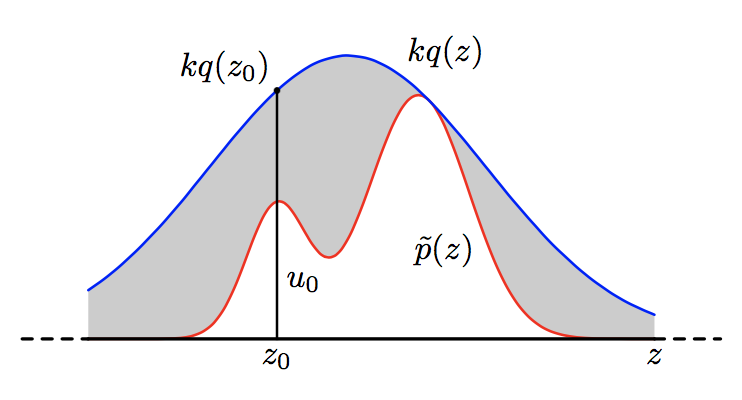
\includegraphics[scale=0.35]{rej_sampling.png}
  \caption{
    Rejection Sampling.
  }
  \end{figure}
  \begin{itemize}
    \item \textbf{Proposal distribution $q(z)$:} We first introduce
    \textit{proposal distribution}, from which we can readily draw samples.
    \begin{equation}
      q(z)
    \end{equation}
    \item \textbf{Bound Constant $k$:} We next introduce a constant $k$
    whose value is chosen such that
    \begin{equation}
      kq(z) \geq \tilde{p}(z) \quad \forall z
    \end{equation}
  \end{itemize}
\end{frame}

\begin{frame}{Rejection Sampling}
  \begin{figure}
  \centering
  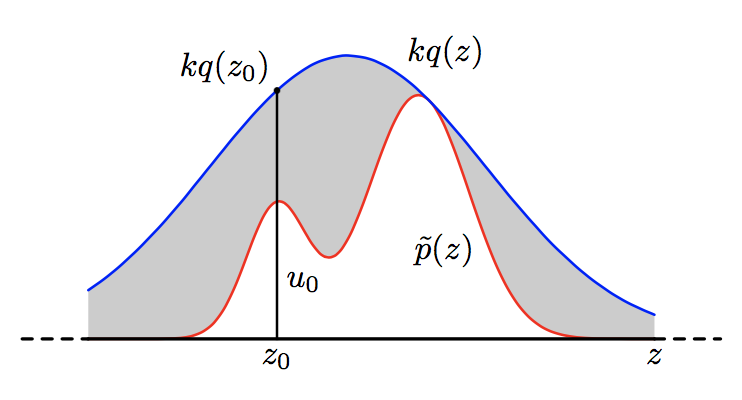
\includegraphics[scale=0.35]{rej_sampling.png}
  \caption{
    Rejection Sampling.
  }
  \end{figure}
  \textbf{Drawing sample} \\
  \begin{enumerate}
    \item Generate a number $z_0$ from the distribution $q(z)$.
    \item Generate a number $u_0$ from the uniform distribution over $[0, kq(z_0)]$.
    \item If $u_0 > \tilde{p}(z_0)$ then the sample is rejected, otherwise accepted.
  \end{enumerate}

  \textbf{The acceptance rate}
  \begin{equation}
    \begin{split}
      p(\textrm{accept}) &= \int \{\tilde{p}(z)/kq(z)\} q(z) \mathrm{d}z \\
      &= \frac{1}{k} \int \tilde{p}(z) \mathrm{d}z
    \end{split}
  \end{equation}
\end{frame}

\begin{frame}{Adaptive Rejection Sampling}
  \textbf{Motivation}\\
  \begin{itemize}
    \item In many instances where we might wish to apply rejection sampling,
    it proves difficult to determine a suitable analytical form for the
    envelope distribution $q(z)$.
    \item How about constructing the envelope function $q(z)$ on the fly
    based on measured values of the distribution $p(z)$.
  \end{itemize}

  \textbf{Settings}\\
  \begin{itemize}
    \item $p(z)$ is log-concave.
    \item The function $\ln p(z)$ and its gradient are evaluated at some
    initial set of grid points, and the intersections of the resulting tangent
    lines are used to construct the envelope function.
    \begin{figure}
    \centering
    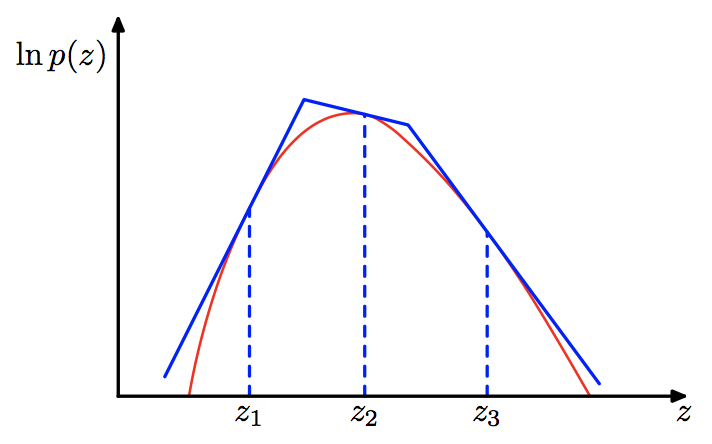
\includegraphics[scale=0.3]{log_env_func.png}
    \caption{
      log envelope function.
    }
    \end{figure}
  \end{itemize}
\end{frame}

\begin{frame}{Adaptive Rejection Sampling}
  \textbf{envelope function}\\
  \begin{itemize}
    \item Because the log envelope distribution is a succession of linear functions,
    and hence the envelope distribution itself comprises a piecewise, smooth
    exponential distribution of the form
    \begin{equation}
      q(z) = k_i\lambda_i \exp {\{ -\lambda_i (z - z_i) \}}
      \quad \textrm{where} \quad \textrm{interval}(z_i)
    \end{equation}
  \end{itemize}

  \textbf{Sampling step} \\
  \begin{enumerate}
    \item A sample valuse is drawn from the envelope distribution, let the
    sample be drawn at $z'$.
    \item If accepted, it will be a sample drawn from the desired distribution.
    \item If the sample is rejected, a new line is evaluated at the
    corresponding position $z'$, and the log envelope function (and
    eventually envelope function) is thereby refined.
  \end{enumerate}
\end{frame}

\begin{frame}{Conclusion to Rejection Sampling}
  \textbf{Conclusions} \\
  \begin{itemize}
    \item The log concave constraint can be vanished simply by following
    each rejection sampling step with a Metropolis-Hastings step (section
    11.2), giving rise to \textit{adaptive rejection metropolis} sampling.
    \item That is, clearly, for rejection sampling to be of practical value,
    we required that the comparison function be close to the required
    distribution so that the rate of rejection is kept to minimum.
  \end{itemize}
  \textbf{Limitations} \\
  \begin{itemize}
    \item For more practical examples, where the desired distribution may be
    multimodal and sharply peaked, it will be extremely difficult to find
    a good proposal distribution and comparison function. (e.g. Gaussian cover)
    \item Furthermore, the exponential decrease of acceptance rate with
    dimensionality is a generic feature of rejection sampling.
  \end{itemize}
\end{frame}

\subsection{Importance Sampling}
\begin{frame}{Importance Sampling}
  \textbf{Motivation} \\
  \begin{itemize}
    \item Only wish to evaluate the expectation, not the samples itselves.
    \item Discretize whole $\mathbfit{z}$-space into a uniform grid and
    evaluate the integration. (c.f. Riemannian sum)
    \begin{equation}
      \mathbb{E}[f] \approx \sum_{l=1}^{L} p(\mathbfit{z}^{(l)})f(\mathbfit{z}^{(l)}).
    \end{equation}
  \end{itemize}

  \textbf{Concerns}\\
  \begin{itemize}
    \item An obvious problem, however, is that the number of terms in the summation grows
    exponentially with the dimensionality of $\mathbfit{z}$.
    \item Only relatively small regions of $\mathbfit{z}$ space has probability.
    \item So this first motivation is very inefficient.
    \item We therefore introduce a proposal distribution $q(z)$.

  \end{itemize}
\end{frame}

\begin{frame}{Importance Sampling}
  \textbf{Approximation} \\
  \begin{itemize}
    \item We can appoximate $\mathbb{E}[f]$ as follows
    \begin{equation}
      \begin{split}
        \mathbb{E}[f]
        &= \int f(\mathbfit{z})p(\mathbfit{z}) \mathrm{d}\mathbfit{z}
         = \int f(\mathbfit{z}) \frac{p(\mathbfit{z})}{q(\mathbfit{z})} q(\mathbfit{z}) \mathrm{d}\mathbfit{z} \\
        &\approx \frac{1}{L} \sum_{l=1}^{L} \frac{p(\mathbfit{z}^{(l)})}{q(\mathbfit{z}^{(l)})} f(\mathbfit{z}^{(l)})
         =       \frac{1}{L} \sum_{l=1}^{L} r_l f(\mathbfit{z}^{(l)})
      \end{split}
    \end{equation}
    where $r_l = \frac{p(\mathbfit{z}^{(l)})}{q(\mathbfit{z}^{(l)})}$ are knwon as
    \textit{importance weights}.
  \end{itemize}

  \textbf{Normalzation constant} \\
  \begin{itemize}
    \item In practical sense,
    \begin{equation}
      \begin{split}
            p(\mathbfit{z}) &= \tilde{p}(\mathbfit{z})/Z_p \\
            q(\mathbfit{z}) &= \tilde{q}(\mathbfit{z})/Z_q
      \end{split}
    \end{equation}
    where $Z_p$ and $Z_q$ are unknown.
    \item The approximation is then given by
    \begin{equation}
      \mathbb{E}[f]
      \approx \frac{Z_q}{Z_p} \frac{1}{L} \sum_{l=1}^{L} \frac{\tilde{p}(\mathbfit{z}^{(l)})}{\tilde{q}(\mathbfit{z}^{(l)})} f(\mathbfit{z}^{(l)})
      =       \frac{Z_q}{Z_p} \frac{1}{L} \sum_{l=1}^{L} \tilde{r}_l f(\mathbfit{z}^{(l)})
    \end{equation}
  \end{itemize}
\end{frame}

\begin{frame}{Importance Sampling}
  \begin{itemize}
    \item The ratio of normalization constants $Z_p$ and $Z_q$ can be
    approximated with same sample set
    \begin{equation}
      \frac{Z_p}{Z_q}
      = \frac{1}{Z_q} \int \tilde{p}(\mathbfit{z}) \mathrm{d}\mathbfit{z}
      = \int \frac{\tilde{p}(\mathbfit{z})}{\tilde{q}(\mathbfit{z})} q(\mathbfit{z}) \mathrm{d}\mathbfit{z}
      \approx \frac{1}{L} \sum_{l=1}^{L} \tilde{r}_l
    \end{equation}
    \item The approximation of $\E[f]$ is therefore given by
    \begin{equation}
      \E[f] \approx \sum_{l=1}^{L} w_l f(\mathbfit{z}^{(l)})
    \end{equation}
    where
    \begin{equation}
      w_l
      = \frac{\tilde{r}_l}{\sum_{m} \tilde{r}_m}
      = \frac{\tilde{q}(\mathbfit{z}^{(l)})/q(\mathbfit{z}^{(l)})}{\sum_m \tilde{q}(\mathbfit{z}^{(m)})/q(\mathbfit{z}^{(m)})}
    \end{equation}
    which implies that the success of the importance sampling approach depends
    crucially on how well the sampling distribution $q(\mathbfit{z})$ matches
    the desired distribution $p(\mathbfit{z})$.
  \end{itemize}
\end{frame}

\begin{frame}{Importance Sampling}
  \textbf{Limitations and Hazards}
  \begin{itemize}
    \item If, as is often the case,
    \begin{enumerate}
      \item $p(z)f(z)$ is strongly varying i.e., $q(z)$ is not tight as much
      as we desired.
      \item Significant proportion of its mass concentrated over relatively
      small regions of $z$ space.
      \item The set ${\{r_l\}}$ may be therefore dominated by a few weights
      having large values.
      \item Thus the effective sample size can be much smaller than the
      apparent sample size $L$.
    \end{enumerate}

    \item The extreme case is where none of the samples falls in the regions
    where $p(z)f(z)$ is large. Just consider the case where the function
    $p(z)f(z)$ is sharply peaked in some small regions of $z$ space.
  \end{itemize}

  \textbf{Conclusion}
  \begin{itemize}
    \item Hence a major drawback of the importance sampling method is the
    potential to produce results that are arbitrarily in error and with no
    diagnostic indication.
    \item This also highlights a key requirement for the sampling distribution
    $q(z)$, namely that it should not be small or zero in regions where $p(z)$
    may be significant.
  \end{itemize}

  \textbf{Further study}
  \begin{itemize}
    \item Likelihood weighted sampling
    \item Self-importance sampling
  \end{itemize}
\end{frame}

\subsection{SIP}
\begin{frame}{Sampling-importance-resampling}
  \textbf{Motivation}
  \begin{itemize}
    \item Importance sampling approach only gives approximation
    to expectation, not samples.
    \item Rejection sampling approach gives samples but it requires
    to determine the constant $k$ with desirable acceptance rate.
  \end{itemize}

  \textbf{Concepts:} There are two stages to the scheme.
  \begin{enumerate}
    \item $L$ samples $\mathbfit{z}^{(l)}$ are drawn from $q(\mathbfit{z})$.
    \item $w_l$ are constructed using (23).
    \item A second set of $L$ samples is drawn from the discrete
    distribution $(\mathbfit{z}^{(1)}, \ldots, \mathbfit{z}^{(L)})$ with
    probability given by the weights $(w_1, \ldots, w_L)$.
  \end{enumerate}

  \textbf{Intuition}
  \begin{itemize}
    \item Let us consider the approximation
    \begin{equation}
      \int f(\mathbfit{z}) \frac{p(\mathbfit{z})}{q(\mathbfit{z})} q(\mathbfit{z}) \mathrm{d}\mathbfit{z}
      \approx \frac{1}{L} \sum_{l=1}^{L} \frac{p(\mathbfit{z}^{(l)})}{q(\mathbfit{z}^{(l)})} f(\mathbfit{z}^{(l)})
      \approx \int f(\mathbfit{z}) \frac{p(\mathbfit{z})}{q(\mathbfit{z})} \mathrm{d}\mathbfit{z}
    \end{equation}
    where $r_l = \frac{p(\mathbfit{z}^{(l)})}{q(\mathbfit{z}^{(l)})}$.
    \item Consider then what is the role of $w_l$
    \begin{equation}
      w_l = \frac{\tilde{r}_l}{\sum_{m} \tilde{r}_m}
    \end{equation}
  \end{itemize}
\end{frame}

\subsection{Sampling and the EM algorithm}
\begin{frame}{Monte Carlo EM algorithm}
  \begin{itemize}
    \item Between E step and M step we must evalute the complete log likelihood
    given by
    \begin{equation}
      Q(\boldsymbol{\theta},\boldsymbol{\theta}^{\textrm{old}})
      = \int p(\mathbf{Z}|\mathbf{X},\boldsymbol{\theta}^{\textrm{old}})
      \ln p(\mathbf{Z},\mathbf{X}|\boldsymbol{\theta})
      \mathrm{d}\mathbf{Z}
    \end{equation}
    which can be approximated by sampling methods as follows
    \begin{equation}
      Q(\boldsymbol{\theta},\boldsymbol{\theta}^{\textrm{old}})
      = \frac{1}{L} \sum_{l=1}^{L} \ln p(\mathbf{Z}^{(l)}, \mathbf{X} | \boldsymbol{\theta})
    \end{equation}
    \item This procedure is called Monte Carlo EM algorithm.
    \item A particular instance of the Monte Carlo EM algorithm, called
    stochastic EM, arises if we consider a finite mixture model, and draw
    just one sample at each E step.
  \end{itemize}
\end{frame}

\begin{frame}{IP algorithm}
  \begin{itemize}
    \item When we move from a maximum likelihood approach to a full Bayesian
    treatment, marginalization is required over the posterior distribution
    $p(\boldsymbol{\theta}|\mathcal{D})$ of the parameter.
    \item Furthermore, we shall suppose that drawing samples from the posterior
    distribution $p(\boldsymbol{\theta}|\mathcal{D})$ is computationally
    difficult.
    \item \textbf{I-step:}
    For some case where there exists latent variable $\mathbf{Z}$
    as follows
    \begin{equation}
      p(\mathbf{Z}|\mathcal{D})
      = \int p(\mathbf{Z|\boldsymbol{\theta}, \mathcal{D}})
      p(\boldsymbol{\theta}|\mathcal{D}) \mathrm{d} \boldsymbol{\theta},
    \end{equation}
    let first draw a sample $\boldsymbol{\theta}^{(l)}$ from the current
    estimate for $p(\boldsymbol{\theta}|\mathcal{D})$, and then draw a
    sample $\mathbf{Z}^{(l)}$ from $p(\mathbf{Z|\boldsymbol{\theta}^{(l)}, \mathcal{D}})$.
    \item \textbf{P-step:}
    Using the sample $\mathbf{Z}^{(l)}$, approximate $p(\boldsymbol{\theta}|\mathcal{D})$
    as follows
    \begin{equation}
      p(\boldsymbol{\theta}|\mathcal{D}) \approx
      \frac{1}{L} \sum_{l=1}^{L} p(\boldsymbol{\theta}|\mathbf{Z}^{(l)}, \mathcal{D}).
    \end{equation}
    \item Note that we are making a (somewhat artificial) distinction between
    parameters $\boldsymbol{\theta}$ and hidden variables $\mathbf{Z}$. From
    now on, we blur this distinction and focus simply on the problem of drawing
    samples from a given posterior distribution.
  \end{itemize}
\end{frame}

\begin{frame}{Summary and Limitations}
  \begin{itemize}
    \item At the heart of the Bayesian inference is ``marginalization.''
    Therfore, the ability to integrate analytically complex and high
    dimensional functions is extremely important in Bayesian statistics.
    \item Sampling methods allows us to sample from posterior distribution
    directly, and obtain sample estimates of the quantities of interests.
    \item With high dimensionality, however, the sampling methods what
    we've discussed so far still have severe limitations.
    \item e.g., guassian enveloping function in rejection sampling.
    \item e.g., Scattered clusters in importance sampling.
  \end{itemize}
\end{frame}

\section{Markov Chain}
\subsection{Markov Chain}
\begin{frame}{Markov Chain; Definition}
  Before discussing MCMC methods, it is fair to study some general and useful
  properties of Markov chains in some detail. We only deals with first-order
  Markov chain in this chapter which is defined by
  \begin{definition}
    A first-order Markov Chain is defined to be a series of \textbf{random variables}
    \begin{equation}
      \mathbfit{z}^{(1)}, \ldots, \mathbfit{z}^{(M)}
    \end{equation}
    satisfying the Markov property given by
    \begin{equation*}
      p(\mathbfit{z}^{(m+1)}|\mathbfit{z}^{(1)}, \ldots, \mathbfit{z}^{(m)})
      = p(\mathbfit{z}^{(m+1)}|\mathbfit{z}^{(m)})
    \end{equation*}
  \end{definition}
  which also can be represented as a directed graph in the form of a chain.
  And the finite-dimensional (here, it stands for time dimension) is given by
  \begin{equation}
    P (\mathbfit{z}^{(1)}, \ldots, \mathbfit{z}^{(M)})
  \end{equation}

\end{frame}

\begin{frame}{Markov Chain; Examining the state space}
  \textit{General definition of Stochastic process}
  \begin{equation}
    X : (\Omega, \mathcal{F}) \rightarrow (S^{\infty},\mathcal{E}^{\infty})
  \end{equation}
  where $(S, \mathcal{E})$ is state space on which $X^{(n)}$'s are defined as
  follows
  \begin{equation}
    X^{(n)} :  (\Omega, \mathcal{F}) \rightarrow (S, \mathcal{E})
  \end{equation}

  \textit{The random variable from State space to Sampling space}
  The stochastic process, or discrete-time Markov chain, have countable
  state space $S$. To simplify the notation and focus on the sample itself
  we introduce the random vector maps original state $S$ to $\mathbf{z}$ which
  is equiprobable, $D$-dimensional space.
  \begin{equation}
    \mathbf{z}^{(n)}: (S, \mathcal{E}) \rightarrow (\mathbf{z}, \mathcal{A})
  \end{equation}
  where $\mathcal{A}$ is a $\sigma$-algebra of $\mathbf{z}$.
\end{frame}


\begin{frame}{Markov Chain; Properties}
  \begin{itemize}
    \item \textit{Initial state}: $\mathbfit{z}^{(0)}$
    \item \textit{Transition probability}:
    \begin{equation}
      T_m(\mathbfit{z}^{(m)},\mathbfit{z}^{(m+1)})
      := p(\mathbfit{z}^{(m+1)}|\mathbfit{z}^{(m)})
    \end{equation}
    \item \textit{Time homogenuity}:
    Time-homogeneous Markov chains (or stationary Markov chains) are processes
    where
    \begin{equation}
      T_m(\mathbfit{z}^{(m)},\mathbfit{z}^{(m+1)})
      = T_n(\mathbfit{z}^{(n)},\mathbfit{z}^{(n+1)})
      \quad \forall m, n
    \end{equation}
    \item \textit{Invariant distribution:}
    \begin{equation}
      p(\mathbfit{z}) = \sum_{\mathbfit{z}'} T(\mathbfit{z}',\mathbfit{z}) p(\mathbfit{z}')
    \end{equation}
    \item \textit{Detailed balance:}
    \begin{equation}
      p(\mathbfit{z}) T(\mathbfit{z},\mathbfit{z}')
      = p(\mathbfit{z}') T(\mathbfit{z}',\mathbfit{z})
    \end{equation}
  \end{itemize}
\end{frame}

\begin{frame}{Markov Chain; properties}
  \textbf{Properties}
  From the definition and the specification of the first-order Markov chain,
  we can examine some useful properties.
  \begin{itemize}
    \item \textit{Reducibility}:
    A Markov chain is said to be irreducible if it is possible to get
    to any state from any state. The accessibility can be defined by
    \begin{equation}
      P(\mathbfit{z}_{n} | \mathbfit{z}_{m}) > 0 \quad \forall n, m
    \end{equation}
    \item \textit{Periodicity}:
    A state $n$ has period $p$ if any return to state $n$ must occur in
    multiples of $p$ time steps. If $p = 1$, then the state is said to
    be \textit{aperiodic}.
    \item \textit{Recurrent}:
    A state $n$ is said to be \textit{transient} if, given that we start
    in state $n$, there is a non-zero probability that we will never
    return to $n$. State $n$ is \textit{recurrent} (or persistent) if
    it is not transient.
    \item \textit{Ergodicity}:
    The Markov chain is called ergodic if it is irreducible, and its
    states are positive recurrent and aperiodic.
  \end{itemize}
\end{frame}

\subsection{Markov Chain for MCMC}
\begin{frame}{Markov Chain for MCMC}
  \textbf{Our goal} is still to generate a sample from $p(\mathbfit{z})$.
  \begin{itemize}
    \item A standard Markov chain Monte Carlo approach is to construct
    an \textbfit{ergodic} Markov chain with a stationary distribution.
  \end{itemize}
  The main properties underpinning the MCMC method, to accomplish our goal,
  are followings.
  \begin{itemize}
    \item \textit{Time reversible property}
    \begin{equation}
      \sum_{\mathbfit{z}'} p(\mathbfit{z}') T(\mathbfit{z}',\mathbfit{z})
      = \sum_{\mathbfit{z}'} p(\mathbfit{z}) T(\mathbfit{z},\mathbfit{z}')
      = p(\mathbfit{z}) \sum_{\mathbfit{z}'} T(\mathbfit{z},\mathbfit{z}')
      = p(\mathbfit{z})
    \end{equation}
    where $p(\mathbfit{z})$ is invariant distribution.

    \item \textit{Existing and unique stationary distribution} \\
    Any chain which is \textit{irreducible} and \textit{aperiodic} will
    have a unique stationary distribution.

    \item \textit{Ergodic property}
    \begin{equation}
      p(\mathbfit{z}^{(m)}) \rightarrow p(\mathbfit{z})
      \quad \textrm{as} \quad
      m \rightarrow \infty
    \end{equation}
  \end{itemize}
\end{frame}

\begin{frame}{Markov Chain for MCMC\cite{MCMC:1998:RSS}}
  \begin{enumerate}
    \item A Markov chain with stationary distribution $p(\mathbfit{z})$ is
    called \textit{time reversible} (or simply \textit{reversible}) if its
    transition kernel $T_m(\mathbfit{z}^{(m)},\mathbfit{z}^{(m+1)})$ is
    such that it exhibits \textit{detailed balance}, i.e.
    \begin{equation}
      p(\mathbfit{z}) T(\mathbfit{z},\mathbfit{z}')
      = p(\mathbfit{z}') T(\mathbfit{z}',\mathbfit{z}).
    \end{equation}
    This essentially means that the chain would look the same whether you
    ran it forwards in time or backwards. The behaviour of reversible chains
    is well understood, and it is a desirable property for any MCMC transition
    kernel to have, since any transition kernel for which \textit{detailed balance}
    holds will have stationary distribution $p(\mathbfit{z})$.

    \item Any chain which is \textit{irreducible} and \textit{aperiodic} will
    have a unique stationary distribution, and that the $t$-step transition
    kernel will `converge' to that stationary distribution as $t \rightarrow \infty$.
    See Meyn and Tweedie (1993).

    \item A Markov chain is \textit{ergodic} if,
    given realizations ${\{ \mathbfit{z}^{(m)}: m = 0, 1, \ldots \}}$
    from the chain, typical asymptotic results include the distributional
    convergence of the realizations. That is, the distribution of the state
    of the chain at time $m$ converges to the stational distribution
    $p(\mathbfit{z})$ as $m \rightarrow \infty$.
    \begin{equation}
      p(\mathbfit{z}^{(m)}) \rightarrow p(\mathbfit{z})
      \quad \textrm{as} \quad
      m \rightarrow \infty
    \end{equation}
  \end{enumerate}
\end{frame}

\section{Markov Chain Monte Carlo}
\subsection{MCMC: Introduction}
\begin{frame}{MCMC: Introduction}
  \textbf{Motivation: Limitation of Basic Samplings}
  \begin{itemize}
    \item In the previous section, we discussed the rejection sampling and
    importance sampling strategies for evaluating expectations of functions,
    and we saw that they suffer from severe limitations particularly in
    spaces of high dimensionality.
  \end{itemize}

  \textbf{Intuition: Markov Chain Monte Carlo}
  \begin{itemize}
    \item General strategy which allows sampling from a large class of
    distribution (based on the mechanism of Markov chains)
    \item It also uses a proposal distribution to generate samples from
    another distribution.
    \item Introduces state, denoted by $\tau$, and remember the previous
    informration, a sample, $\mathbfit{z}^{(\tau)}$
    \item The proposal distribution then depends on the current state:
    $q(\mathbfit{z}|\mathbfit{z}^{(\tau)})$
  \end{itemize}
\end{frame}

\subsection{MCMC Algorithms}
\begin{frame}{MCMC Algorithms}
  \textbf{Goal and Requirement}
  \begin{itemize}
    \item \textbf{Goal:} to generate a sample from $p(\mathbfit{z})$
    \item \textbf{Requirement 1: stationary distribution} \\
    A markov chain where $p(\mathbfit{z})$ is invariant.
    \item \textbf{Requirement 2: ergodicity property} \\
    With requirement 1, $p(\mathbfit{z}^{(m)}) \rightarrow p(\mathbfit{z})$ as $m \rightarrow \infty$
  \end{itemize}

  \textbf{Sampling Step}
  \begin{enumerate}
    \item Remembering the current sample $\mathbfit{z}^{(\tau)}$, generate
    a candidate sample $\mathbfit{z}^{*}$ from a proposal distribution
    $q(\mathbfit{z}|\mathbfit{z}^{(\tau)})$.
    \item Accept the sample according to the criterion.
    \item If the candidate sample is accepted, then
    $\mathbfit{z}^{(\tau+1)} \leftarrow \mathbfit{z}^{*}$,
    otherwise
    $\mathbfit{z}^{(\tau+1)} \leftarrow \mathbfit{z}^{(\tau)}$.
  \end{enumerate}

  \textbf{Note that}
  \begin{itemize}
    \item The sequence of samples $\mathbfit{z}^{(1)}, \mathbfit{z}^{(1)}, \ldots$
    are strongly dependent to previous sample due to its sequential sampling.
    We therefore chose only $M$th samples to ensure the independence.
  \end{itemize}
\end{frame}

\begin{frame}{Metropolis-Hastings Algorithm}
  \textbf{Acceptance function:}
  \begin{equation}
    A_k(\mathbfit{z}^{*}, \mathbfit{z}^{(\tau)})
    = \min_k
    \left(
      1,
      \frac{\tilde{p}(\mathbfit{z}^{*}) q_k(\mathbfit{z}^{(\tau)}|\mathbfit{z}^{*})}
      {\tilde{p}(\mathbfit{z}^{(\tau)}) q_k(\mathbfit{z}^{*}|\mathbfit{z}^{(\tau)})}
    \right)
  \end{equation}
  Here $k$ labels the members of the set of possible transitions being
  considered.

  \textbf{Rejection criteria:}
  For $\mathbfit{z}^{*}$ from the proposal distribution $q(\mathbfit{z}^{*}|\mathbfit{z}^{(\tau)})$,
  Consider the function $A_k(\mathbfit{z}^{*}, \mathbfit{z}^{(\tau)})$.
  Here the transition probabilit is given by
  \begin{equation}
    q(\mathbfit{z}^{*}|\mathbfit{z}^{(\tau)})A_k(\mathbfit{z}^{*}, \mathbfit{z}^{(\tau)})
  \end{equation}

  \textbf{Validation of limiting distribution}
  \begin{equation}
    \begin{split}
      p(\mathbfit{z}) q_k(\mathbfit{z}'|\mathbfit{z}) A_k(\mathbfit{z}', \mathbfit{z})
      &= \min(p(\mathbfit{z}) q_k(\mathbfit{z}'|\mathbfit{z}), p(\mathbfit{z}') q_k(\mathbfit{z}|\mathbfit{z}'))  \\
      &= \min(p(\mathbfit{z}') q_k(\mathbfit{z}|\mathbfit{z}'), p(\mathbfit{z}) q_k(\mathbfit{z}'|\mathbfit{z}))  \\
      &= p(\mathbfit{z}') q_k(\mathbfit{z}|\mathbfit{z}') A_k(\mathbfit{z}, \mathbfit{z}')
    \end{split}
  \end{equation}
\end{frame}

\begin{frame}{Metropolis Algorithm}
  \textbf{Symmetry specification:} $q_k(\mathbfit{z}|\mathbfit{z}') = q_k(\mathbfit{z}'|\mathbfit{z})$
  \textbf{Acceptance function:}
  \begin{equation}
    A(\mathbfit{z}^{*}, \mathbfit{z}^{(\tau)})
    = \min
    \left(
      1,
      \frac{\tilde{p}(\mathbfit{z}^{*})}
      {\tilde{p}(\mathbfit{z}^{(\tau)})}
    \right)
  \end{equation}
  where $q(\mathbfit{z}_A|\mathbfit{z}_B) = q(\mathbfit{z}_B|\mathbfit{z}_A)$
  for all $A$ and $B$.
  \\[1.0\baselineskip]

  \textbf{Rejection criterion}
  \begin{equation}
    \begin{split}
      \textrm{Reject: } &A_(\mathbfit{z}^{*}, \mathbfit{z}^{(\tau)}) \leq u \\
      \textrm{Accept: } &A_(\mathbfit{z}^{*}, \mathbfit{z}^{(\tau)}) > u
    \end{split}
  \end{equation}
  where $u$ is randomly picked from uniform distribution $U(0,1)$.

  \textbf{Validation of limiting distribution}
  \begin{equation}
    \begin{split}
      p(\mathbfit{z}) q_k(\mathbfit{z}'|\mathbfit{z}) A_k(\mathbfit{z}', \mathbfit{z})
      &= q_k(\mathbfit{z}'|\mathbfit{z} ) \min{\left\{ p(\mathbfit{z} ), p(\mathbfit{z}') \right\}}  \\
      &= q_k(\mathbfit{z} |\mathbfit{z}') \min{\left\{ p(\mathbfit{z}'), p(\mathbfit{z}) \right\}}  \\
      &= p(\mathbfit{z}') q_k(\mathbfit{z}|\mathbfit{z}') A_k(\mathbfit{z}, \mathbfit{z}')
    \end{split}
  \end{equation}
\end{frame}

\begin{frame}{Gibbs Sampling}
  \begin{figure}
  \centering
  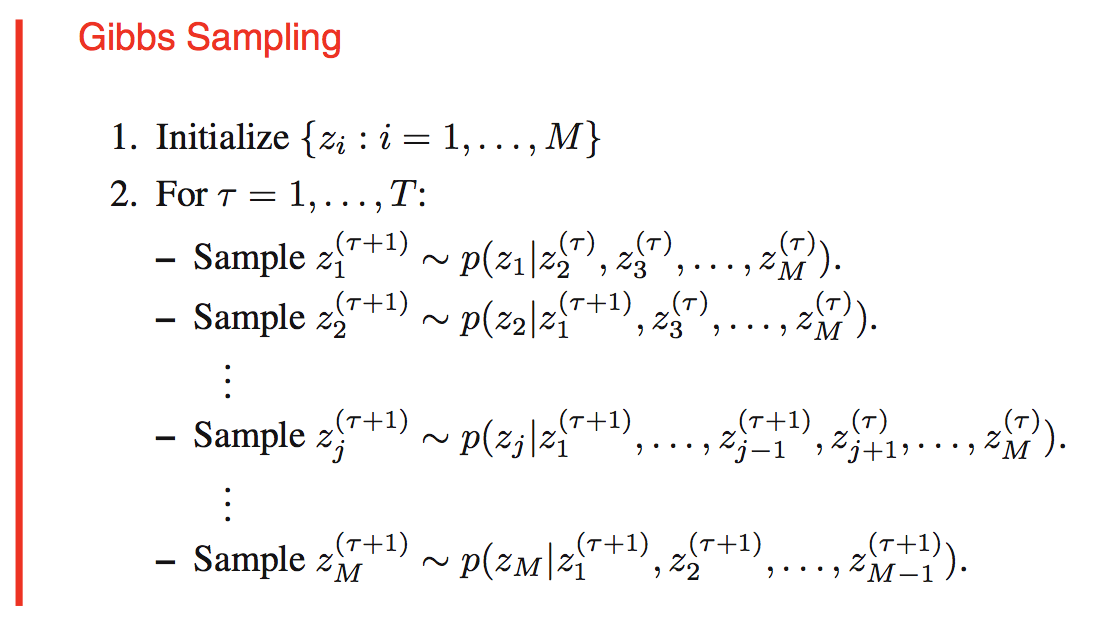
\includegraphics[scale=0.45]{gibbs_sampling.png}
  \caption{
    Gibbs Sampling.
  }
  \end{figure}
\end{frame}

\begin{frame}{Gibbs Sampling}
  \textbf{Acceptance function:}
  \begin{equation}
    A_(\mathbfit{z}^{*}, \mathbfit{z})
    =
      \frac{p(\mathbfit{z}^{*}) q_k(\mathbfit{z}|\mathbfit{z}^{*})}
      {p(\mathbfit{z}^{(\tau)}) q_k(\mathbfit{z}^{*}|\mathbfit{z})}
    =
    \frac{p(z_k^{*}|\mathbfit{z}_{-k}^{*}) p(\mathbfit{z}_{-k}^{*}) p(z_k|\mathbfit{z}_{-k}^{*})}
    {p(z_k|\mathbfit{z}_{-k}) p(\mathbfit{z}_{-k}) p(z_k^{*}|\mathbfit{z}_{-k})}
  \end{equation}
  where $\mathbfit{z}_{-k} = \mathbfit{z}^{*}_{-k}$
  \\[1.0\baselineskip]

  \textbf{Validation of equilibrium distribution $p$}
  \begin{equation}
    p(z_i = z_i^{(\tau + 1)}) = T(z_i = z_i^{(\tau)}, z_i = z_i^{(\tau + 1)}) p(z_i = z_i^{(\tau)})
  \end{equation}
  where $T = p(z_i|\mathbfit{z}_{-i})$.
\end{frame}

\begin{frame}{Slice Sampling}
  \textbf{Motivation}
  \begin{itemize}
    \item In Metropolis-Hastings Algorithm, If the step size is too small, the
    result is slow decorrelation due to random walk behaviour, whereas if it is
    too large the result is inefficiency due to a high rejection rate.
  \end{itemize}

  \textbf{Concept}
  \begin{itemize}
    \item adaptive step size that is automatically adjusted to match the
    characteristics of the distribution.
  \end{itemize}

  \begin{figure}
  \centering
  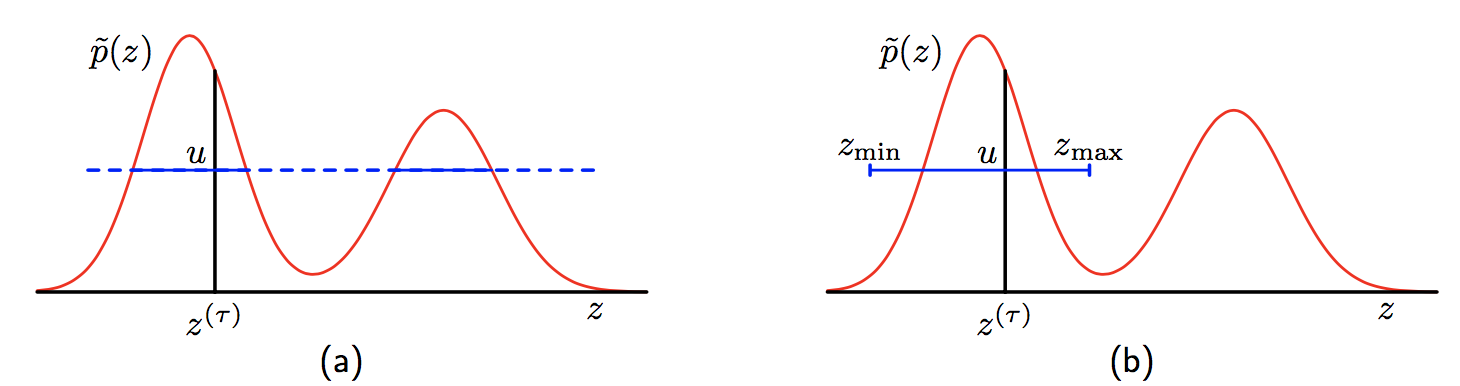
\includegraphics[scale=0.4]{slice_sampling.png}
  \caption{
    Slice Sampling.
  }
  \end{figure}
\end{frame}

%%%%%%%%%%%%%%%%%%%%%%%%%%%%%%%%%%%%%%%%%%%%%%%%%%%%%%%%%%%%%%%%%%%%%
\end{document}
%%%%%%%%%%%%%%%%%%%%%%%%%%%%%%%%%%%%%%%%%%%%%%%% DOCUMENT start
